Before we can run any experiment, we have to pin down the task so
precisely that a machine can carry it out and we can score it
objectively. Vague tasks give vague answers; a task with concrete
inputs, runnable outputs, and hidden tests gives crisp, checkable
answers.

A well-designed exam question is the model. It's not enough to say
``write a program about numbers.'' We need: exactly what the input is,
exactly what the program should do, and exactly how to check if it's
right. That's what we're about to define.

\section{The task}\label{the-task}

The model receives a \textbf{natural-language specification} of a
programming task and must produce a \textbf{Python program} that solves
it. That program is then executed against hidden tests.

\begin{figure}
\centering
\pandocbounded{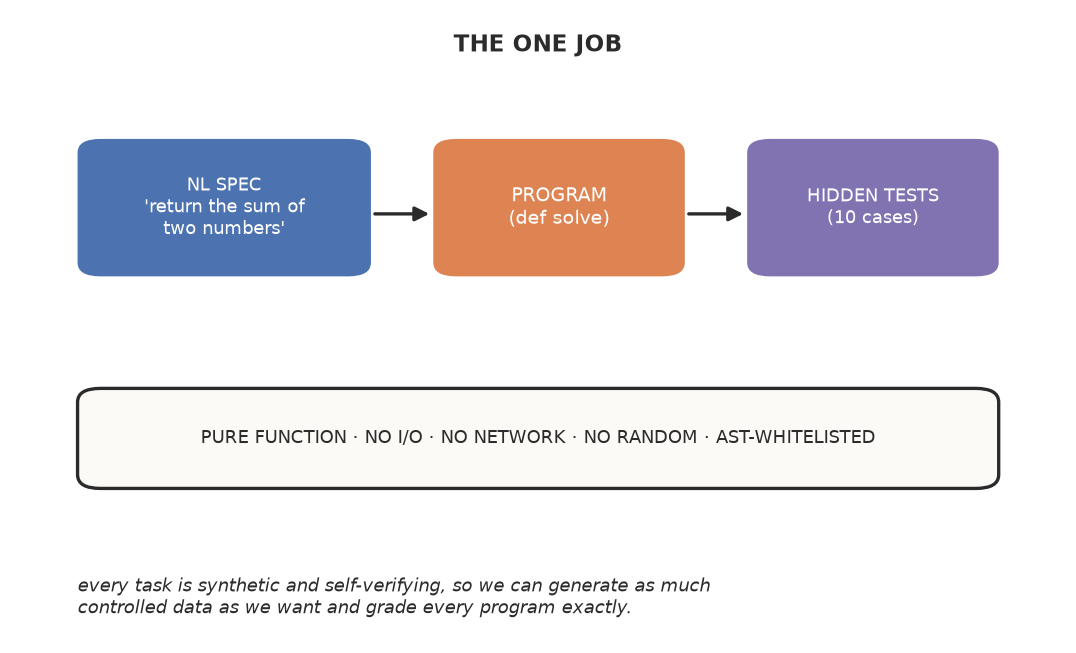
\includegraphics[keepaspectratio,alt={The one job},width=\maxwidth{\textwidth},keepaspectratio]{figures/fig_task.png}}
\caption{The one job}
\end{figure}

The contract is simple: a natural-language specification in, a program
out, and a set of hidden tests to grade it against. Everything else
follows from it.

Concretely, the model sees something like:

\begin{quote}
``Write a function that takes two numbers, a and b, and returns their
sum.''
\end{quote}

and must produce:

\begin{Shaded}
\begin{Highlighting}[]
\KeywordTok{def}\NormalTok{ solve(a, b):}
    \ControlFlowTok{return}\NormalTok{ a }\OperatorTok{+}\NormalTok{ b}
\end{Highlighting}
\end{Shaded}

We score it by running that program against a set of hidden test cases
(inputs with expected outputs) and checking whether the program's output
matches, semantically, for every case.

\section{The task schema}\label{the-task-schema}

Every task is described by a small, formal schema --- the ground truth
that drives everything. The key insight is that \textbf{one semantic
record generates all three} things we need: the reference program, the
natural-language spec, and the hidden tests. That way there is no drift
between ``what the task is'' and ``how we ask for it'' and ``how we test
it.''

The semantic core captures the operation and its arguments:

\begin{Shaded}
\begin{Highlighting}[]
\FunctionTok{\{}
  \DataTypeTok{"operation"}\FunctionTok{:} \StringTok{"add"}\FunctionTok{,}
  \DataTypeTok{"args"}\FunctionTok{:} \OtherTok{[}\FunctionTok{\{}\DataTypeTok{"name"}\FunctionTok{:} \StringTok{"a"}\FunctionTok{,} \DataTypeTok{"type"}\FunctionTok{:} \StringTok{"int"}\FunctionTok{\}}\OtherTok{,} \FunctionTok{\{}\DataTypeTok{"name"}\FunctionTok{:} \StringTok{"b"}\FunctionTok{,} \DataTypeTok{"type"}\FunctionTok{:} \StringTok{"int"}\FunctionTok{\}}\OtherTok{]}\FunctionTok{,}
  \DataTypeTok{"output\_type"}\FunctionTok{:} \StringTok{"int"}
\FunctionTok{\}}
\end{Highlighting}
\end{Shaded}

From that single record, the teacher generates: 1. the reference Python
(\texttt{def\ solve(a,b):\ return\ a+b}), 2. a natural-language
specification (in one of several phrasings), 3. a set of hidden tests
(ordinary, zero, negative, boundary, large cases).

\section{The pure-function
constraint}\label{the-pure-function-constraint}

For the pilot we constrain the generated programs to be \textbf{pure
functions}. No side effects, no file I/O, no randomness. This makes
evaluation deterministic and unambiguous: for a given input, there is
one correct output. It is a deliberate simplification, and it is exactly
what makes the task cleanly measurable.

\section{Hidden tests}\label{hidden-tests}

The hidden tests are the heart of evaluation. Each task carries an
independent set of test cases designed to catch real errors, not just a
single happy path. For an arithmetic task we include ordinary values,
zero, negatives, boundary values, and large-magnitude values. The tests
are generated independently of the reference program's \emph{logic} ---
computed from the semantics, not copied from the solution --- so that a
model that merely memorizes the reference still can't predict the exact
test suite.

\section{The success criterion}\label{the-success-criterion}

For a single problem, the success criterion is:

\begin{quote}
\textbf{Problem-level hidden-test pass@1} --- did the one program the
model produced pass \emph{every} hidden test for that problem, under
deterministic/greedy decoding?
\end{quote}

This is deliberately strict. A program that passes 7 of 8 hidden tests
\emph{fails} the problem. That strictness is what keeps the measurement
honest: we are not measuring ``close,'' we are measuring ``correct.''

\section{Why this specific task}\label{why-this-specific-task}

Natural-language-to-Python is a good laboratory task precisely because
it has everything a controlled experiment needs:

\begin{itemize}
\tightlist
\item
  \textbf{Deterministic.} Same spec, same program, same tests.
\item
  \textbf{Executable.} We run real Python and compare real outputs.
\item
  \textbf{Objectively scorable.} Pass/fail, no judge-subjectivity.
\item
  \textbf{Synthetic.} We can generate as much controlled data as we
  want.
\item
  \textbf{Controllable difficulty.} We can escalate from \texttt{a+b} to
  compounded operations.
\item
  \textbf{Compositional splits.} We can train on pieces and test on
  unseen combinations.
\item
  \textbf{Memorization tests.} We can plant canaries and check for exact
  reproduction.
\item
  \textbf{Auditable.} We can inspect the exact generated program and run
  shortcut audits.
\end{itemize}

The model could not ask for a clearer job. Now we have to build the
tools that let us run and score it: a controlled world, a teacher, a
judge, and rivals.
